% https://ask.latexstudio.net/ask/question/7543.html
\documentclass[tikz,border=8pt]{standalone}
\usepackage[svgnames]{xcolor}
\usepackage{fourier}
\usetikzlibrary{arrows.meta,calc,positioning,shadows,shapes.geometric,shapes.symbols}
\begin{document}
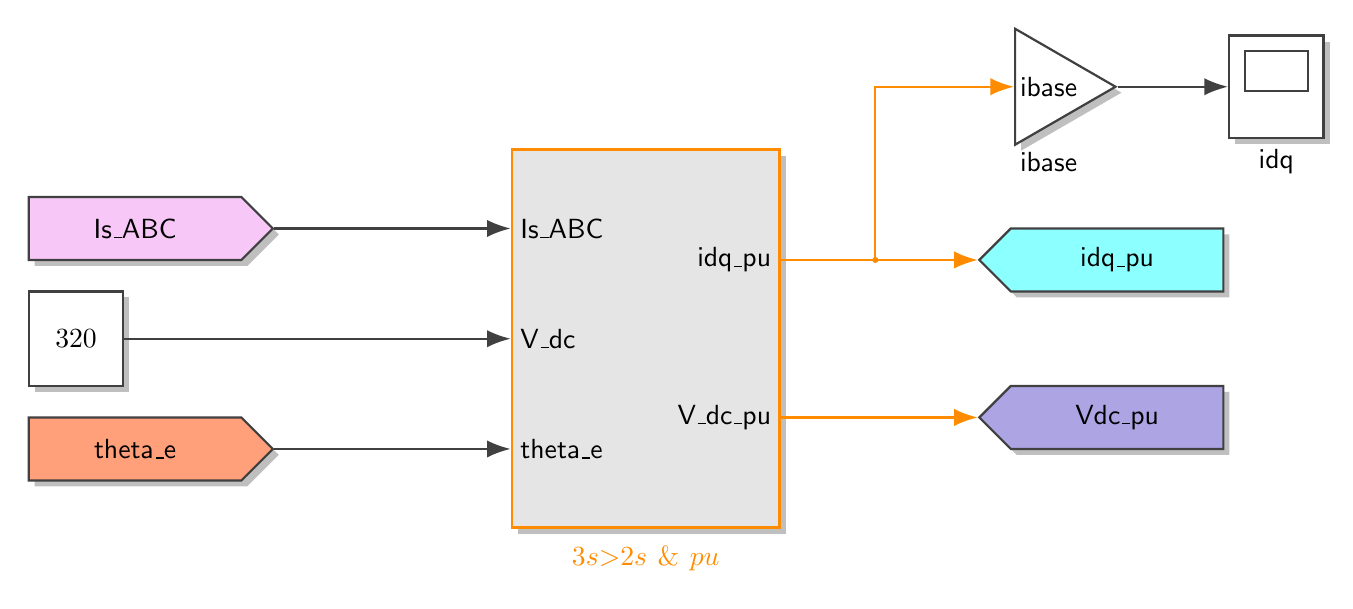
\begin{tikzpicture}[
  font=\sffamily,=Latex,
  line/.style={wire,draw=black!75},
  orange line/.style={wire,draw=DarkOrange},
  wire/.style={line width=.8pt,-{Latex[length=3mm,width=2.2mm]}},
  component/.style={draw=black!75,line width=.8pt,fill=white,drop shadow},
  tag/.style={component,signal,signal to=#1,minimum width=31mm,minimum height=8mm,inner xsep=4mm},
  block/.style={component,draw=DarkOrange,fill=gray!20,line width=.9pt,minimum width=34mm,minimum height=48mm},
  constant/.style={component,minimum size=12mm},
  gain/.style={component,regular polygon,regular polygon sides=3,shape border rotate=-90,minimum size=17mm},
  display/.style={component,minimum width=12mm,minimum height=13mm}
]
\node[block] (system) {};
\node[tag=east,fill=Violet!45,anchor=east] (isabc) at ([xshift=-30mm,yshift=14mm]system.west) {Is\_ABC};
\node[constant,anchor=west] (dc) at (isabc.west |- system.west) {$320$};
\node[tag=east,fill=LightSalmon,anchor=east] (theta) at ([xshift=-30mm,yshift=-14mm]system.west) {theta\_e};
\node[anchor=west] at ([yshift=14mm]system.west) {Is\_ABC};
\node[anchor=west] at (system.west) {V\_dc};
\node[anchor=west] at ([yshift=-14mm]system.west) {theta\_e};
\node[anchor=east] at ([yshift=10mm]system.east) {idq\_pu};
\node[anchor=east] at ([yshift=-10mm]system.east) {V\_dc\_pu};
\node[DarkOrange,anchor=north,font=\bfseries] at ([yshift=-1mm]system.south) {$3s{>}2s\ \&\ pu$};
\node[tag=west,fill=Cyan!45,anchor=west] (idqpu) at ([xshift=25mm,yshift=10mm]system.east) {idq\_pu};
\node[tag=west,fill=SlateBlue!55,anchor=west] (vdcpu) at ([xshift=25mm,yshift=-10mm]system.east) {Vdc\_pu};
\coordinate (branch) at ($(system.east)+(12mm,10mm)$);
\node[gain] (ibase) at ([xshift=22mm,yshift=22mm]branch) {};
\node at (ibase) {ibase};
\node[below=2mm of ibase] (ibaselabel) {ibase};
\node[display,right=14mm of ibase] (display) {};
\node[rectangle,draw=black!75,line width=.7pt,minimum width=8mm,minimum height=5mm] at ([yshift=2mm]display.center) {};
\node at (ibaselabel -| display) {idq};
\draw[line] (isabc.east) -- ([yshift=14mm]system.west);
\draw[line] (dc.east) -- (system.west);
\draw[line] (theta.east) -- ([yshift=-14mm]system.west);
\draw[orange line] ([yshift=10mm]system.east) -- (idqpu.west);
\draw[orange line] ([yshift=-10mm]system.east) -- (vdcpu.west);
\fill[DarkOrange] (branch) circle (1.1pt);
\draw[orange line] (branch) |- (ibase.west);
\draw[line] (ibase.east) -- (display.west);
\end{tikzpicture}
\end{document}
